%
% main.tex
%
% Copyright (C) 2022 by SpaceLab.
%
% TTC 2.0 Module
%
% This work is licensed under the Creative Commons Attribution-ShareAlike 4.0
% International License. To view a copy of this license,
% visit http://creativecommons.org/licenses/by-sa/4.0/.
%

%
% \brief Main file.
%
% \author Gabriel Mariano Marcelino <gabriel.mm8@gmail.com>
% \author Miguel Boing <miguelboing13@gmail.com>
%
% \version 0.1.0
%
% \date 2022/07/28
%

\documentclass{beamer}

\usepackage{presentation}

\title[Presentation]{SpaceLab TTC 2.0}
\author[SpaceLab]{Miguel Boing, Gabriel M. Marcelino}
\institute[]{SpaceLab - UFSC}
\date{2022 August 24}

\hypersetup
{
    pdfauthor	= {SpaceLab},
    pdfsubject	= {TTC 2.0 module},
    pdftitle	= {\title},
    pdfkeywords	= {Nanosatellites, CubeSats, TMTC}
}

\begin{document}

    %
% titlepage.tex
%
% Copyright (C) 2021 by SpaceLab.
%
% TTC 2.0 Documentation
%
% This work is licensed under the Creative Commons Attribution-ShareAlike 4.0
% International License. To view a copy of this license,
% visit http://creativecommons.org/licenses/by-sa/4.0/.
%

%
% \brief Title page.
%
% \author Gabriel Mariano Marcelino <gabriel.mm8@gmail.com>
%
% \institution Universidade Federal de Santa Catarina (UFSC)
%
% \version 0.0.1
%
% \date 2021/04/01
%

\begin{titlepage}

\thispagestyle{empty}

\begin{flushleft}
SLB-TTC2-DOC-v0.1
\end{flushleft}

\vspace{1cm}

\begin{figure}[!ht]
    \begin{flushleft}
        
\includegraphics[width=7cm]{figures/spacelab-logo-full-color-rgb-1000px@72ppi.png}
    \end{flushleft}
\end{figure}

\begin{flushleft}
\Huge{\textbf{\thetitle}}
\rule[0pt]{\textwidth}{5pt}
\end{flushleft}

\vspace{0.2cm}

\begin{flushleft}
\textit{\thetitle} \\
\textit{SpaceLab, Universidade Federal de Santa Catarina, Florianópolis - Brazil}
\end{flushleft}

\vfill
\vfill

\begin{flushright}
May 2021
\end{flushright}

\end{titlepage}

    %
% contents.tex
%
% Copyright (C) 2022 by SpaceLab.
%
% TTC 2.0 Module
%
% This work is licensed under the Creative Commons Attribution-ShareAlike 4.0
% International License. To view a copy of this license,
% visit http://creativecommons.org/licenses/by-sa/4.0/.
%

%
% \brief Table of contents.
%
% \author Gabriel Mariano Marcelino <gabriel.mm8@gmail.com>
% \author Miguel Boing <miguelboing13@gmail.com>
%
% \version 0.1.0
%
% \date 2022/06/24
%

\begin{frame}
    \frametitle{Summary}
    \tableofcontents
\end{frame}


    \section{Project Overview}

        %
% introduction.tex
%
% Copyright (C) 2021 by SpaceLab.
%
% TTC 2.0 Documentation
%
% This work is licensed under the Creative Commons Attribution-ShareAlike 4.0
% International License. To view a copy of this license,
% visit http://creativecommons.org/licenses/by-sa/4.0/.
%

%
% \brief Introduction chapter.
%
% \author Gabriel Mariano Marcelino <gabriel.mm8@gmail.com>
%
% \institution Universidade Federal de Santa Catarina (UFSC)
%
% \version 0.0.0
%
% \date 2021/04/01
%

\chapter{Introduction} \label{ch:introduction}

.

\cite{test}, \cite{obdh2}

LEO\nomenclature{\textbf{LEO}}{\textit{Low Earth Orbit.}}


    \section{Hardware}

        %
% design.tex
%
% Copyright (C) 2022 by SpaceLab.
%
% TTC 2.0 Critical Design Review
%
% This work is licensed under the Creative Commons Attribution-ShareAlike 4.0
% International License. To view a copy of this license,
% visit http://creativecommons.org/licenses/by-sa/4.0/.
%

%
% \brief Design slides.
%
% \author Gabriel Mariano Marcelino <gabriel.mm8@gmail.com>
% \author Miguel Boing <miguelboing13@gmail.com>
%
% \version 0.1.0
%
% \date 2022/07/28
%


\begin{frame}{Specifications}

    \begin{itemize}
        \item \textbf{Microcontroller}: MSP430F6659/MSP430F5659
        \item \textbf{Clock}: 32 MHz
        \item \textbf{Memories}:
        \begin{itemize}
            \item \textit{RAM}: 64 kB (SRAM)
            \item \textit{Flash}: 512 kB (code)
        \end{itemize}
        \item \textbf{Sensors}: Voltage, current and temperature
        \item \textbf{Modulation}: (G)FSK or (G)MSK
        \item \textbf{Baudrate}: 1200 to 9600 bps
        \item \textbf{Frequency}: 145-146 MHz, 435-438 MHz or 450 MHz bands
        \item \textbf{Protocol}: NGHam
        \item \textbf{Interfaces}: UART, I$^{2}$C and SPI
        \item \textbf{Mass}: 73 g
        \item PC-104 compatible
    \end{itemize}

\end{frame}

% #########################################################################
% #########################################################################

\begin{frame}{Electrical Block Diagram}

    \begin{figure}[!ht]
        \begin{center}
            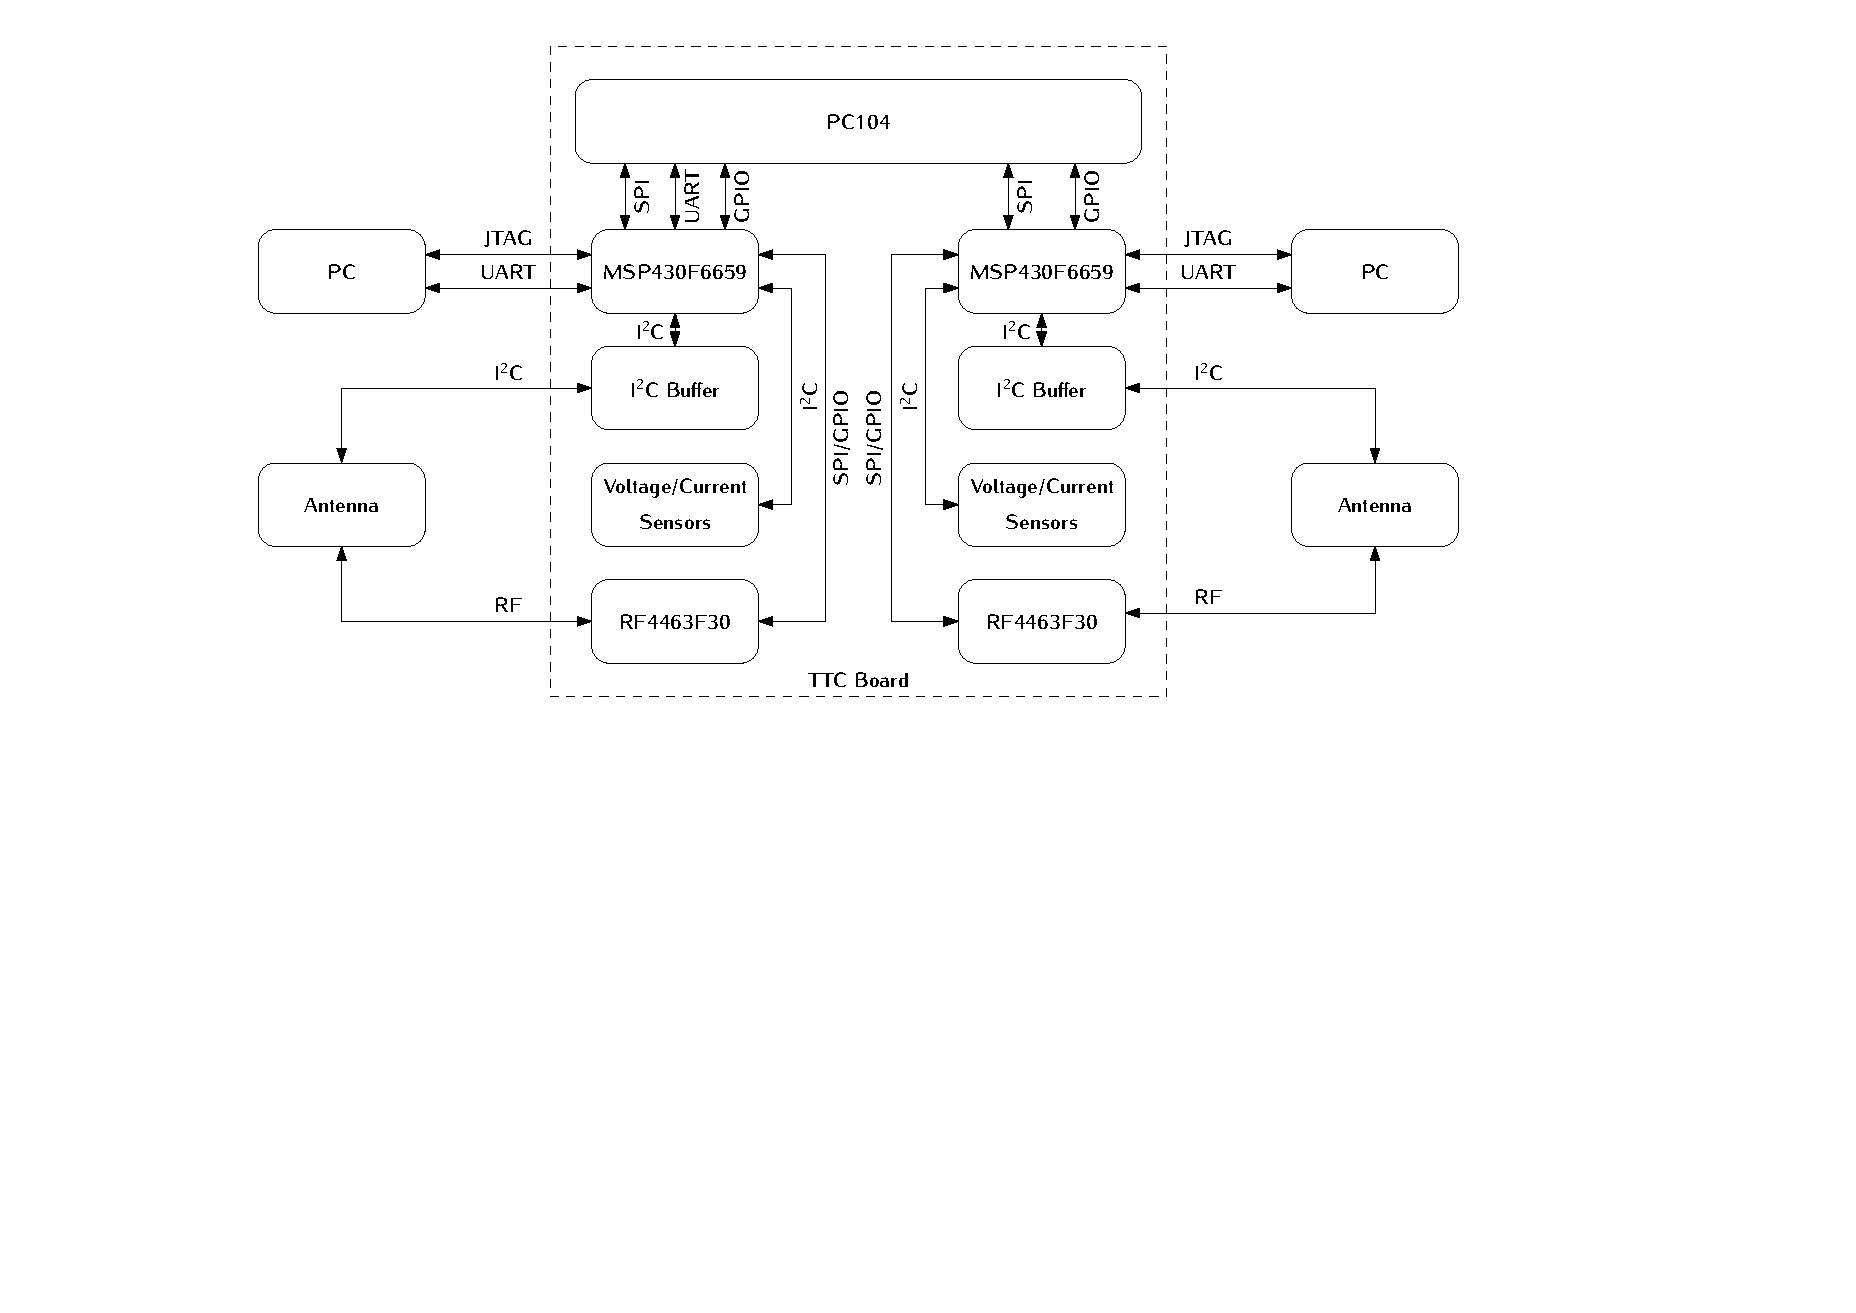
\includegraphics[width=11cm]{figures/hardware_diagram}
        \end{center}
    \end{figure}

\end{frame}

\begin{frame}{Schematics}

    Available at: \href{https://github.com/spacelab-ufsc/ttc2/tree/master/hardware/outputs/board_schematics}{\textcolor{blue}{\underline{https://github.com/spacelab-ufsc/ttc2}}}

    \begin{figure}[!ht]
        \begin{center}
            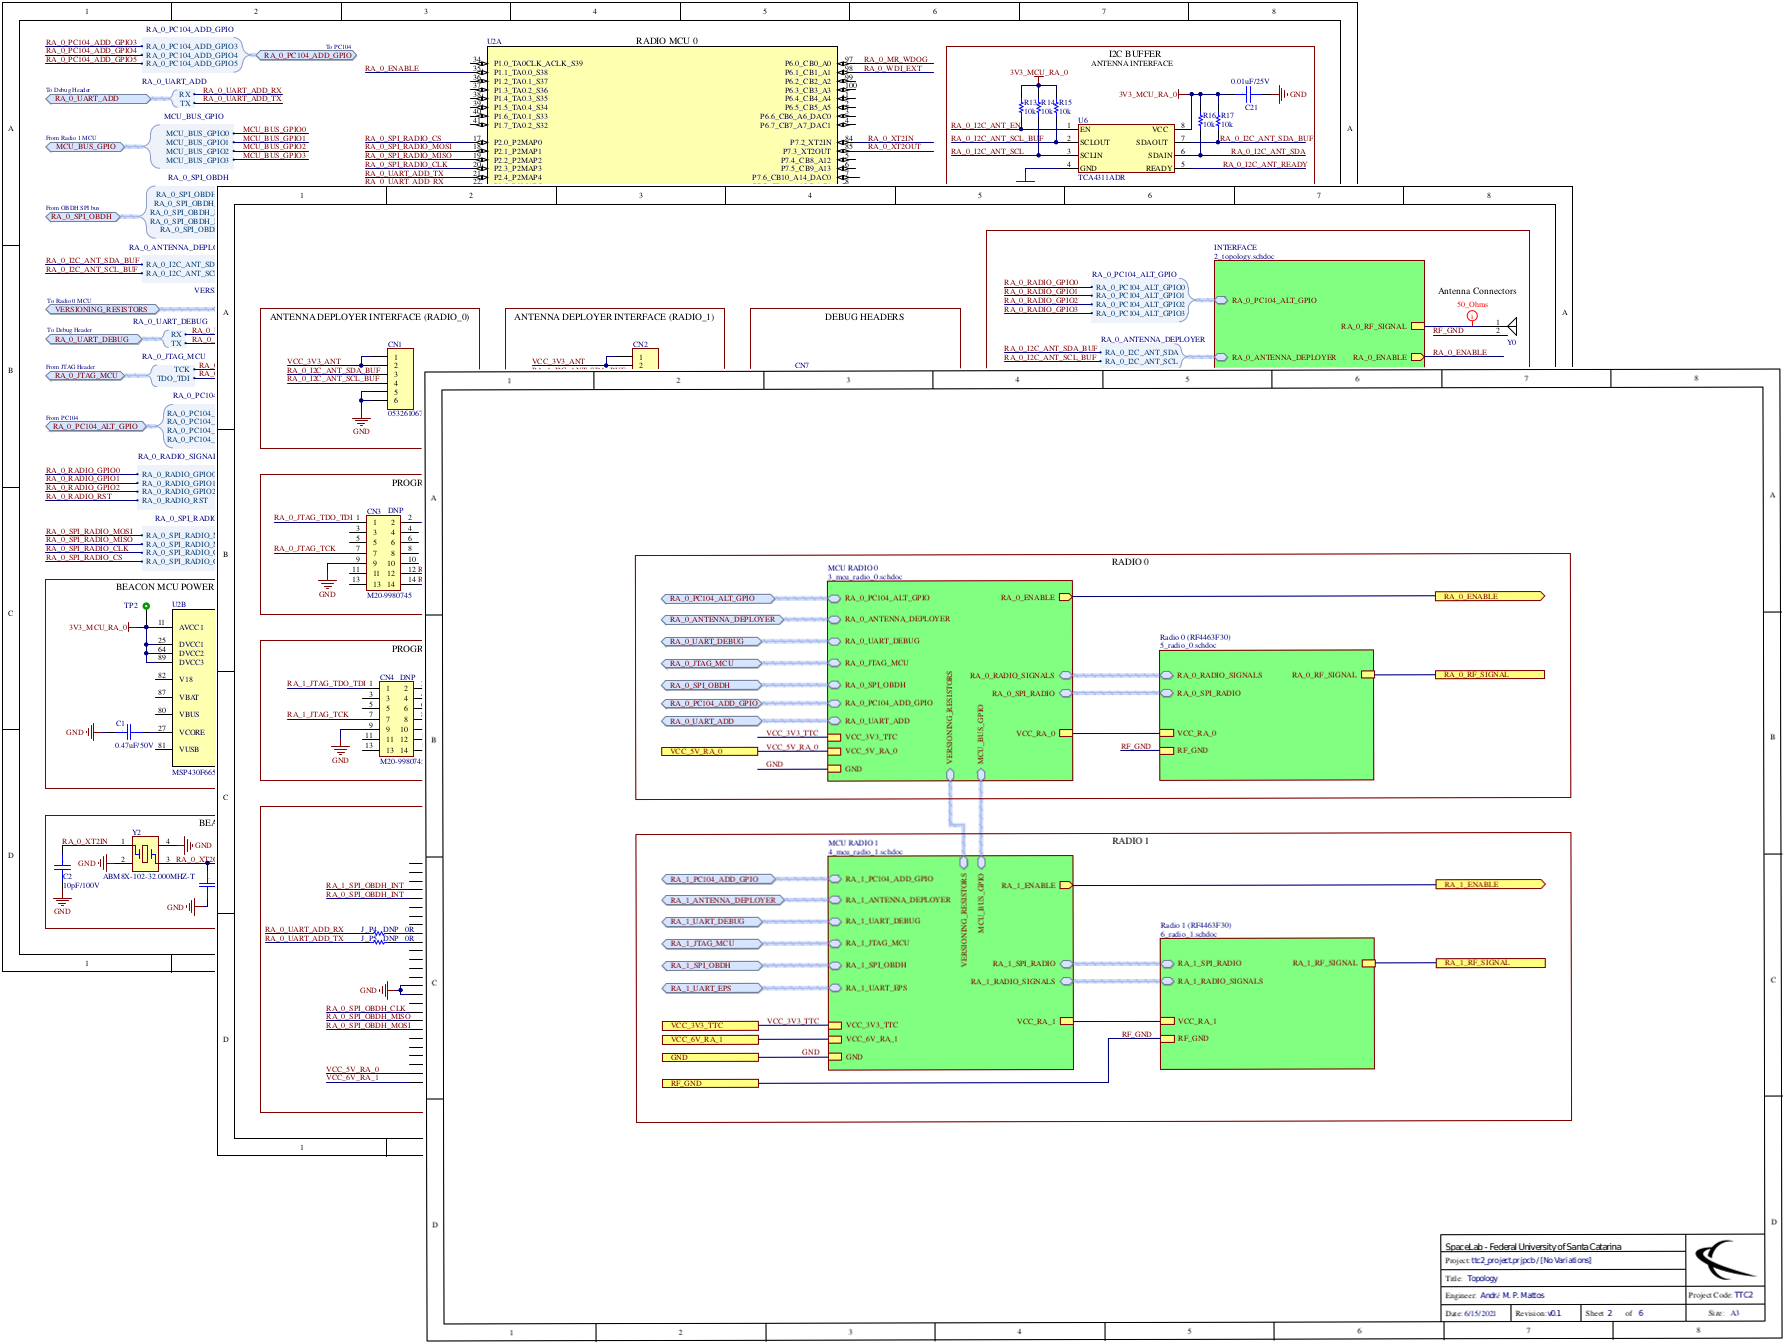
\includegraphics[width=8.5cm]{figures/ttc2-schematics.png}
        \end{center}
    \end{figure}

\end{frame}

\begin{frame}{PCB Layout}

    Available at: \href{https://github.com/spacelab-ufsc/ttc2/tree/master/hardware/sources}{\textcolor{blue}{\underline{https://github.com/spacelab-ufsc/ttc2}}}

    \begin{columns}[t]
        \begin{column}[t]{0.5\textwidth}
            \begin{figure}[!ht]
                \begin{center}
                    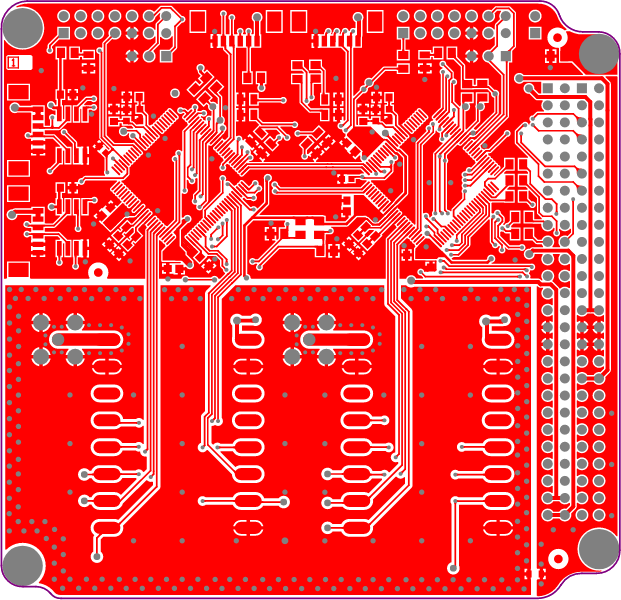
\includegraphics[width=5cm]{figures/ttc2-layout-top.png}
                \end{center}
                \caption{Top side}
            \end{figure}
        \end{column}
        \begin{column}[t]{0.5\textwidth}
            \begin{figure}[!ht]
                \begin{center}
                    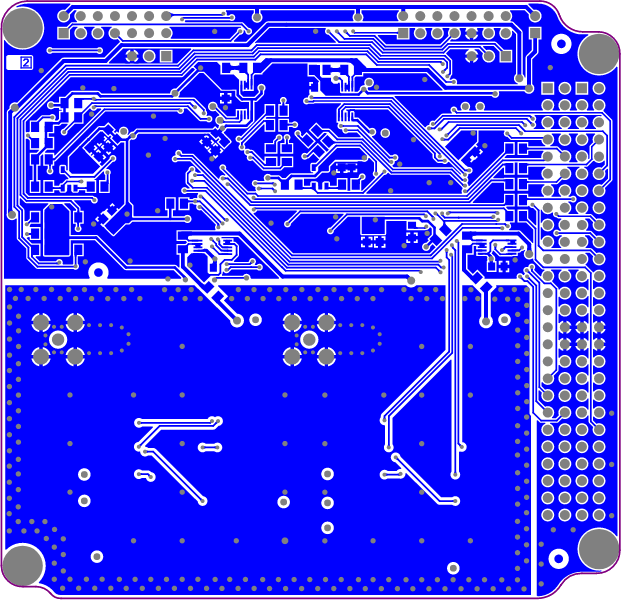
\includegraphics[width=5cm]{figures/ttc2-layout-bottom.png}
                \end{center}
                \caption{Bottom side}
            \end{figure}
        \end{column}
    \end{columns}

\end{frame}

\begin{frame}{3D Model}

    Available at: \href{https://github.com/spacelab-ufsc/ttc2/tree/master/hardware/outputs/board_3dmodels}{\textcolor{blue}{\underline{https://github.com/spacelab-ufsc/ttc2}}}

    \begin{figure}[!ht]
        \begin{center}
            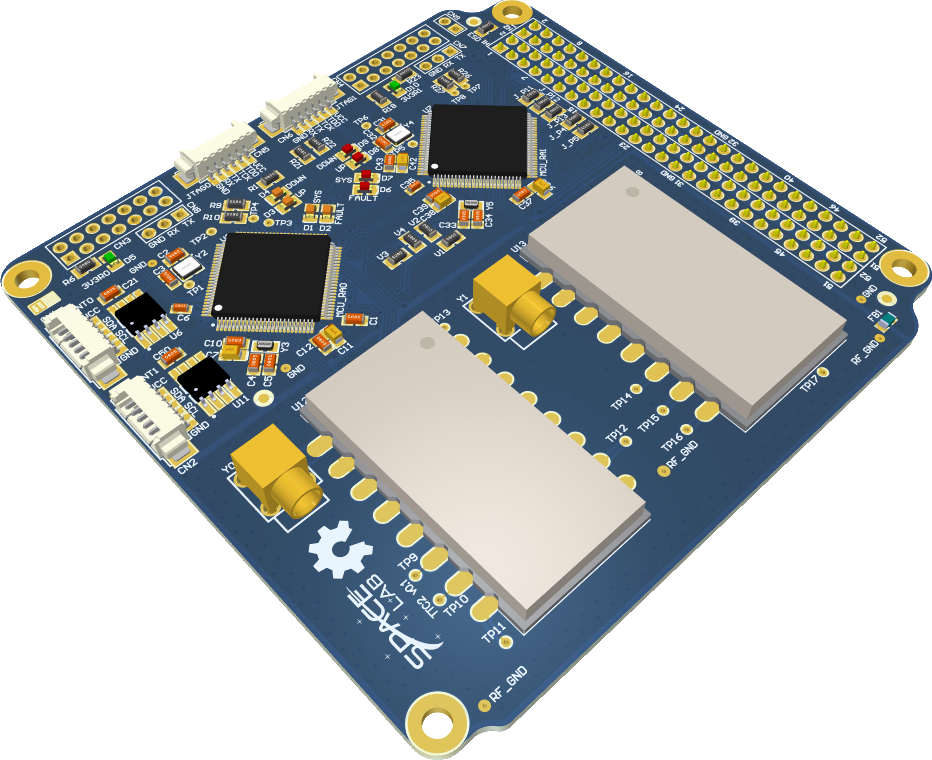
\includegraphics[width=7.5cm]{figures/ttc2_pcb_3d.png}
        \end{center}
    \end{figure}

\end{frame}

% #########################################################################
% #########################################################################

\begin{frame}{Power Consumption}

    \begin{itemize}
        \item Three separated voltage inputs: 3V3, 5V and 6V (microcontrollers and transceivers)
        \vspace{0.5cm}
        \item Power consumption\footnote{For one transceiver (there is two in TTC 2.0)}:
            \begin{itemize}
                \item Stand-by mode $\cong$ 83 mW
                \vspace{0.3cm}
                \item Transmission mode $\cong$ 2800 mW
                \vspace{0.3cm}
                \item Reception mode $\cong$ 163 mW
            \end{itemize}
    \end{itemize}

\end{frame}

% #########################################################################
% #########################################################################

\begin{frame}{Electrical Interfaces: PC-104}

\begin{table}[!h]\tiny
    \centering
    \begin{tabular}{cllll}
        \toprule[1.5pt]
        \textbf{Pin [A-B]} & \textbf{H1A}     & \textbf{H1B}     & \textbf{H2A}  & \textbf{H2B}  \\
        \midrule
        1-2                & -                & -                & -                & -                \\
        3-4                & -                & -                & -                & -                \\
        5-6                & -                & -                & RA\_1\_UART\_RX  & -                \\
        7-8                & GPIO\_6          & GPIO\_7          & RA\_1\_UART\_TX  & GPIO\_0          \\
        9-10               & RA\_1\_SPI\_INT  & RA\_1\_EN        & -                & -                \\
        11-12              & RA\_0\_SPI\_INT  & RA\_0\_EN        & RA\_1\_SPI\_MOSI & RA\_1\_SPI\_CLK  \\
        13-14              & -                & -                & RA\_1\_SPI\_CS   & RA\_1\_SPI\_MISO \\
        15-16              & -                & -                & -                & -                \\
        17-18              & -                & -                & -                & GPIO\_1          \\
        19-20              & -                & GPIO\_2          & -                & GPIO\_3          \\
        21-22              & -                & -                & -                & GPIO\_4          \\
        23-24              & -                & -                & -                & -                \\
        25-26              & -                & -                & -                & -                \\
        27-28              & -                & -                & VCC\_3V3         & VCC\_3V3         \\
        29-30              & GND              & GND              & GND              & GND              \\
        31-32              & GND              & GND              & GND              & GND              \\
        33-34              & -                & -                & -                & -                \\
        35-36              & RA\_0\_SPI\_CLK  & -                & VCC\_3V3\_ANT    & VCC\_3V3\_ANT    \\
        37-38              & RA\_0\_SPI\_MISO & -                & -                & -                \\
        39-40              & RA\_0\_SPI\_MOSI & RA\_0\_SPI\_CS   & -                & -                \\
        41-42              & -                & -                & -                & GPIO\_5          \\
        43-44              & -                & -                & -                & -                \\
        45-46              & -                & -                & -                & -                \\
        47-48              & -                & -                & -                & -                \\
        49-50              & VCC\_5V\_RA\_0   & VCC\_5V\_RA\_0   & -                & -                \\
        51-52              & VCC\_6V\_RA\_1   & VCC\_6V\_RA\_1   & -                & -                \\
        \bottomrule[1.5pt]
    \end{tabular}
    \label{tab:pc104-pins}
\end{table}

\end{frame}

\begin{frame}{Other Electrical Interfaces}

    \begin{table}[!htb]\tiny
        \centering
        \label{tab:icd}
        \begin{tabular}{lccl}
            \toprule[1.5pt]
            \textbf{Connector} & \textbf{Interface} & \textbf{Type} & \textbf{Pins} \\
            \midrule
            \multirow{6}{*}{CN1} & \multirow{6}{*}{I$^{2}$C} & \multirow{6}{*}{PicoBlade} & 3V3 \\
                                 &                           &                            & 3V3 \\
                                 &                           &                            & I2C\_SDA \\
                                 &                           &                            & I2C\_SCL \\
                                 &                           &                            & GND \\
                                 &                           &                            & GND \\
            \midrule
            \multirow{6}{*}{CN2} & \multirow{6}{*}{I$^{2}$C} & \multirow{6}{*}{PicoBlade} & 3V3 \\
                                 &                           &                            & 3V3 \\
                                 &                           &                            & I2C\_SDA \\
                                 &                           &                            & I2C\_SCL \\
                                 &                           &                            & GND \\
                                 &                           &                            & GND \\
            \bottomrule[1.5pt]
        \end{tabular}
    \end{table}

\end{frame}

\begin{frame}{Other Electrical Interfaces}

    \begin{table}[!htb]\tiny
        \centering
        \label{tab:icd}
        \begin{tabular}{lccl}
            \toprule[1.5pt]
            \textbf{Connector} & \textbf{Interface} & \textbf{Type} & \textbf{Pins} \\
            \midrule
            \multirow{14}{*}{CN3} & \multirow{14}{*}{JTAG} & \multirow{14}{*}{Pin Header} & TDO\_TDI \\
                                  &                        &                              & 3V3 \\
                                  &                        &                              & None \\
                                  &                        &                              & None \\
                                  &                        &                              & None \\
                                  &                        &                              & None \\
                                  &                        &                              & TCK \\
                                  &                        &                              & None \\
                                  &                        &                              & GND \\
                                  &                        &                              & None \\
                                  &                        &                              & None \\
                                  &                        &                              & UART\_TX \\
                                  &                        &                              & None \\
                                  &                        &                              & UART\_RX \\

            \bottomrule[1.5pt]
        \end{tabular}
    \end{table}

\end{frame}

\begin{frame}{Other Electrical Interfaces}

    \begin{table}[!htb]\tiny
        \centering
        \label{tab:icd}
        \begin{tabular}{lccl}
            \toprule[1.5pt]
            \textbf{Connector} & \textbf{Interface} & \textbf{Type} & \textbf{Pins} \\
            \midrule
            \multirow{14}{*}{CN4} & \multirow{14}{*}{JTAG} & \multirow{14}{*}{Pin Header} & TDO\_TDI \\
                                  &                        &                              & 3V3 \\
                                  &                        &                              & None \\
                                  &                        &                              & None \\
                                  &                        &                              & None \\
                                  &                        &                              & None \\
                                  &                        &                              & TCK \\
                                  &                        &                              & None \\
                                  &                        &                              & GND \\
                                  &                        &                              & None \\
                                  &                        &                              & None \\
                                  &                        &                              & UART\_TX \\
                                  &                        &                              & None \\
                                  &                        &                              & UART\_RX \\

            \bottomrule[1.5pt]
        \end{tabular}
    \end{table}

\end{frame}

\begin{frame}{Other Electrical Interfaces}

    \begin{table}[!htb]\tiny
        \centering
        \label{tab:icd}
        \begin{tabular}{lccl}
            \toprule[1.5pt]
            \textbf{Connector} & \textbf{Interface} & \textbf{Type} & \textbf{Pins} \\
            \midrule
            \multirow{6}{*}{CN5} & \multirow{6}{*}{JTAG} & \multirow{6}{*}{PicoBlade} & 3V3 \\
                                 &                       &                            & TDO\_TDI \\
                                 &                       &                            & TCK \\
                                 &                       &                            & UART\_TX \\
                                 &                       &                            & UART\_RX \\
                                 &                       &                            & GND \\
            \midrule
            \multirow{6}{*}{CN6} & \multirow{6}{*}{JTAG} & \multirow{6}{*}{PicoBlade} & 3V3 \\
                                 &                       &                            & TDO\_TDI \\
                                 &                       &                            & TCK \\
                                 &                       &                            & UART\_TX \\
                                 &                       &                            & UART\_RX \\
                                 &                       &                            & GND \\
            \midrule
            \multirow{3}{*}{CN7} & \multirow{3}{*}{UART} & \multirow{3}{*}{PinHeader} & TX \\
                                 &                       &                            & RX \\
                                 &                       &                            & GND \\
            \midrule
            \multirow{3}{*}{CN8} & \multirow{3}{*}{UART} & \multirow{3}{*}{PicoBlade} & TX \\
                                 &                       &                            & RX \\
                                 &                       &                            & GND \\
            \midrule
            \multirow{2}{*}{CN9} & \multirow{2}{*}{Jumper} & \multirow{2}{*}{Pin Header} & 3V3 \\
                                 &                         &                      & - \\
            \bottomrule[1.5pt]
        \end{tabular}
    \end{table}

\end{frame}

\begin{frame}{Other Electrical Interfaces}

    \begin{table}[!htb]\tiny
        \centering
        \label{tab:icd}
        \begin{tabular}{lccl}
            \toprule[1.5pt]
            \textbf{Connector} & \textbf{Interface} & \textbf{Type} & \textbf{Pins} \\
            \midrule
            \multirow{2}{*}{Y0} & \multirow{2}{*}{RF} & \multirow{2}{*}{MCX} & RF\_SIGNAL \\
                                &                     &                      & RF\_GND \\
            \midrule
            \multirow{2}{*}{Y1} & \multirow{2}{*}{RF} & \multirow{2}{*}{MCX} & RF\_SIGNAL \\
                                &                     &                      & RF\_GND \\
            \bottomrule[1.5pt]
        \end{tabular}
    \end{table}

\end{frame}

\begin{frame}{Dimensions}

    \begin{figure}[!ht]
        \begin{center}
            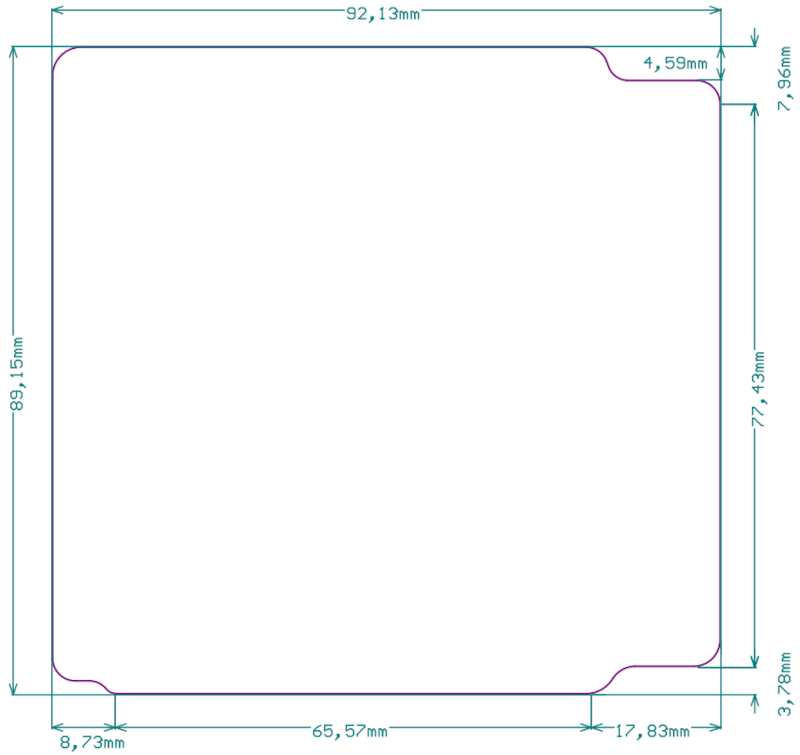
\includegraphics[width=7.5cm]{figures/board-dimensions.png}
        \end{center}
    \end{figure}

\end{frame}

\begin{frame}{Voltage/Current Sensors}

    \begin{itemize}
        \item Voltage, current and power sensor
        \vspace{0.3cm}
        \item Quantity: 4 (one per radio module and one per microncontroller circuit)
        \vspace{0.3cm}
        \item Texas Instruments INA226AQDGSRQ1
        \vspace{0.3cm}
        \item I$^{2}$C Interface
        \vspace{0.3cm}
    \end{itemize}


\end{frame}

\begin{frame}{External Watchdog}

    \begin{itemize}
        \item IC: Texas Instruments TPS3823
        \vspace{0.5cm}
        \item Voltage monitor with a watchdog timer feature
        \vspace{0.5cm}
        \item Timeout period: $1600\ ms$
        \vspace{0.5cm}
        \item Reset period: $100\ ms$
    \end{itemize}

\end{frame}

\begin{frame}{Transceiver}

    \begin{itemize}
        \item \href{https://www.nicerf.com/products/detail/1w-rf-module-rf4463f30.html}{\textcolor{blue}{\underline{NiceRF RF4463F30}}}
        \item Based on \href{https://www.silabs.com/wireless/proprietary/ezradiopro-sub-ghz-ics/device.si4463?tab=specs}{\textcolor{blue}{\underline{Si4463}}} transceiver
        \item Integrated power amplifier and RF switch (single antenna)
        \item Half-Duplex
        \item Output power: 30 dBm
        \item SPI Interface
    \end{itemize}
    \begin{figure}[!ht]
        \begin{center}
            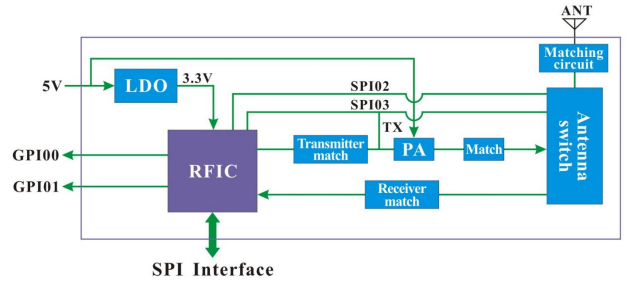
\includegraphics[width=10cm]{figures/rf4463f30-block-diagram.png}
        \end{center}
    \end{figure}

\end{frame}

\begin{frame}{Flight Model Specs. and Preparation}

    \begin{itemize}
        \item \textbf{PCB specs.}: IPC 6012 Class 3
        \vspace{0.3cm}
        \item \textbf{PCB thickness}: 1,6 mm
        \vspace{0.3cm}
        \item \textbf{Material}: TG170 FR-4
        \vspace{0.3cm}
        \item \textbf{Surface finish}: ENIG
        \vspace{0.3cm}
        \item \textbf{Board finish}: Conformal coating application
    \end{itemize}

\end{frame}


    \section{Firmware}

        %
% firmware.tex
%
% Copyright The TTC 2.0 Contributors.
%
% TTC 2.0 Documentation
%
% This work is licensed under the Creative Commons Attribution-ShareAlike 4.0
% International License. To view a copy of this license,
% visit http://creativecommons.org/licenses/by-sa/4.0/.
%

%
% \brief Firmware project chapter.
%
% \author Gabriel Mariano Marcelino <gabriel.mm8@gmail.com>
%
% \version 0.2.0
%
% \date 2021/05/12
%

\chapter{Firmware} \label{ch:firmware}

.

\section{Product tree}

The product tree of the firmware part of the TTC 2.0 module is available in \autoref{fig:product-tree-fw}.

\begin{figure}[!ht]
    \begin{center}
        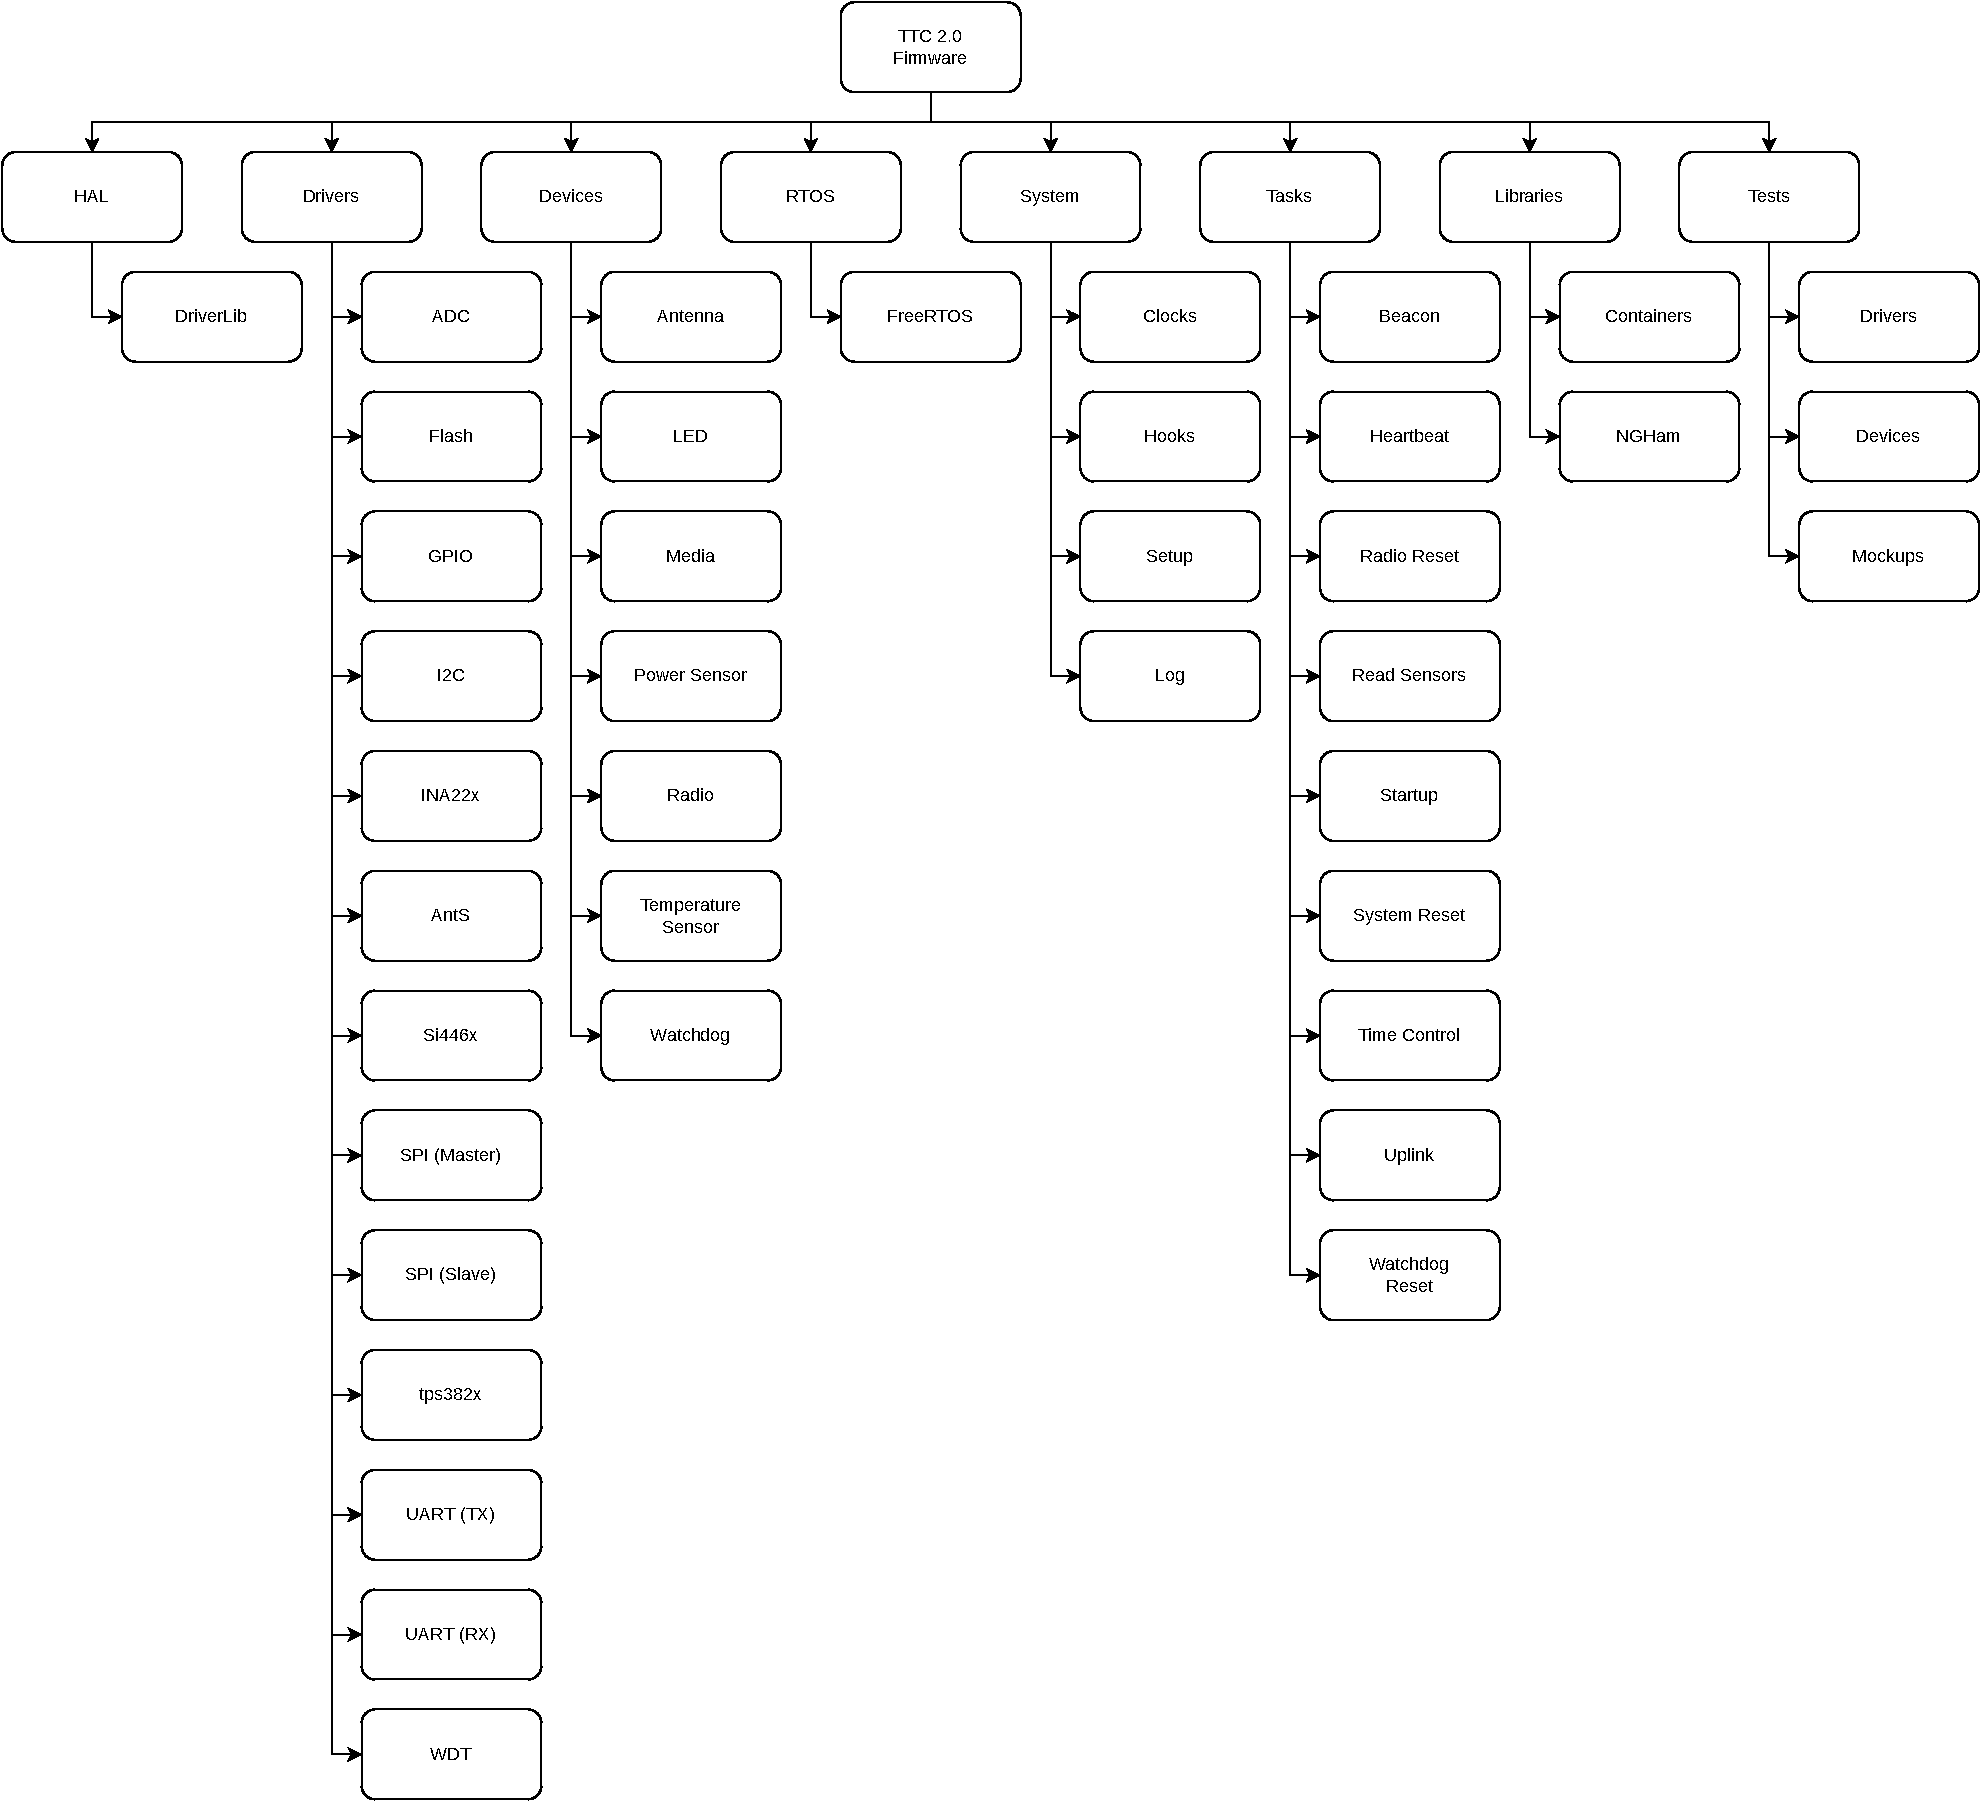
\includegraphics[width=\textwidth]{figures/product-tree-fw.pdf}
        \caption{Product tree of the firmware of the TTC 2.0 module.}
        \label{fig:product-tree-fw}
    \end{center}
\end{figure}

\section{Commands}

The SPI\nomenclature{\textbf{SPI}}{\textit{Serial Peripheral Interface.}} commands of the TTC module are available in \autoref{tab:commands}. All commands are composed by an ID field (1 byte), the content of the command and a checksum at the end of the command (2 bytes). The used checksum algorithm is the CRC16-CCITT\nomenclature{\textbf{CRC}}{\textit{Cyclic Redundancy Check.}} \nomenclature{\textbf{CCITT}}{\textit{Comité Consultatif International Téléphonique et Télégraphique.}} (initial value = 0x0000, polynomial = 0x1021) the value is calculated with the entire packet (ID field + command content).

\begin{table}[!h]
    \centering
    \begin{tabular}{cll}
        \toprule[1.5pt]
        \textbf{ID} & \textbf{Name/Description} & \textbf{Content}\\
        \midrule
        0   & NOP                       & None \\
        1   & Read parameter/variable   & Parameter ID (1B) + Value (4B) + Checksum (2B) \\
        2   & Write parameter/variable  & Parameter ID (1B) + Value (4B) + Checksum (2B) \\
        3   & Transmit packet           & Packet data (1-220B) + Checksum (2B) \\
        4   & Receive packet            & Packet data (1-220B) + Checksum (2B) \\
        \bottomrule[1.5pt]
    \end{tabular}
    \caption{List of commands.}
    \label{tab:commands}
\end{table}

\subsection{Variables and Parameters}

A list of all the variables of TTC with their identification number (ID) and variable type that can be read from the sensors and peripherals is seen in the \autoref{tab:ttc2-variables}.

\begin{longtable}[c]{cL{0.72\textwidth}lc}
    \toprule[1.5pt]
    \textbf{ID} & \textbf{Name/Description} & \textbf{Type} & \textbf{Access} \\
    \midrule
    0   & Device ID (0xCC2A or 0xCC2B)                                      & uint16 & R \\
    1   & Hardware version                                                  & uint8  & R \\
    2   & Firmware version (ex.: ``v1.2.3''' = 0x00010203)                  & uint32 & R \\
    3   & Time counter in millseconds                                       & uint32 & R \\
    4   & Reset counter                                                     & uint16 & R \\
    \multirow{18}{*}{5} & Last reset cause: & \multirow{18}{*}{uint8} & \multirow{18}{*}{R} \\
        & - 0x00 = No interrupt pending                                     &        &  \\
        & - 0x02 = Brownout (BOR)                                           &        &  \\
        & - 0x04 = RST/NMI (BOR)                                            &        &  \\
        & - 0x06 = PMMSWBOR (BOR)                                           &        &  \\
        & - 0x08 = Wakeup from LPMx.5 (BOR)                                 &        &  \\
        & - 0x0A = Security violation (BOR)                                 &        &  \\
        & - 0x0C = SVSL (POR)                                               &        &  \\
        & - 0x0E = SVSH (POR)                                               &        &  \\
        & - 0x10 = SVML\_OVP (POR)                                          &        &  \\
        & - 0x12 = SVMH\_OVP (POR)                                          &        &  \\
        & - 0x14 = PMMSWPOR (POR)                                           &        &  \\
        & - 0x16 = WDT time out (PUC)                                       &        &  \\
        & - 0x18 = WDT password violation (PUC)                             &        &  \\
        & - 0x1A = Flash password violation (PUC)                           &        &  \\
        & - 0x1C = Reserved                                                 &        &  \\
        & - 0x1E = PERF peripheral/configuration area fetch (PUC)           &        &  \\
        & - 0x20 = PMM password violation (PUC)                             &        &  \\
        & - 0x22 to 0x3E = Reserved                                         &        &  \\
    6   & Input voltage of the $\mu$C in mV                                 & uint16 & R \\
    7   & Input current of the $\mu$C in mA                                 & uint16 & R \\
    8   & Temperature of the $\mu$C in K                                    & uint16 & R \\
    9   & Input voltage of the radio in mV                                  & uint16 & R \\
    10  & Input current of the radio in mA                                  & uint16 & R \\
    11  & Temperature of the radio in K                                     & uint16 & R \\
    12  & Last valid command (uplink packet ID)                             & uint8  & R \\
    13  & RSSI of the last valid telecommand                                & uint16 & R \\
    14  & Temperature of the antenna module in K                            & uint16 & R \\
    \multirow{17}{*}{15} & Antenna module status bits:                      & \multirow{17}{*}{uint16} & \multirow{17}{*}{R} \\
        & - Bit 15: The antenna 1 is deployed (0) or not (1)                &        &   \\
        & - Bit 14: Cause of the latest activation stop for antenna 1       &        &   \\
        & - Bit 13: The antenna 1 deployment is active (1) or not (0)       &        &   \\
        & - Bit 11: The antenna 2 is deployed (0) or not (1)                &        &   \\
        & - Bit 10: Cause of the latest activation stop for antenna 2       &        &   \\
        & - Bit 9: The antenna 2 deployment is active (1) or not (0)        &        &   \\
        & - Bit 8: The antenna is ignoring the deployment switches (1) or not (0) &  &   \\
        & - Bit 7: The antenna 3 is deployed (0) or not (1)                 &        &   \\
        & - Bit 6: Cause of the latest activation stop for antenna 3        &        &   \\
        & - Bit 5: The antenna 3 deployment is active (1) or not (0)        &        &   \\
        & - Bit 4: The antenna system independent burn is active (1) or not (0) &    &   \\
        & - Bit 3: The antenna 4 is deployed (0) or not (1)                 &        &   \\
        & - Bit 2: Cause of the latest activation stop for antenna 4        &        &   \\
        & - Bit 1: The antenna 4 deployment is active (1) or not (0)        &        &   \\
        & - Bit 0: The antenna system is armed (1) or not (0)               &        &   \\
    16  & Antenna deployment status (0=never executed, 1=executed)          & uint8  & R \\
    17  & Antenna deployment hibernation (0=never executed, 1=executed)     & uint8  & R \\
    18  & TX enable (0=off, 1=on)                                           & uint8  & R/W \\
    19  & TX packet counter                                                 & uint32 & R \\
    20  & RX packet counter (valid packets)                                 & uint32 & R \\
    21  & TX packets available in the FIFO buffer                           & uint8  & R \\
    22  & RX packets available in the FIFO buffer                           & uint8  & R \\
    23  & Number of bytes of the first available packet in the RX buffer    & uint16 & R \\
    \bottomrule[1.5pt]
    \caption{Variables and parameters of the TTC 2.0.}
    \label{tab:ttc2-variables}
\end{longtable}


    \section{Operation}

        %
% operation.tex
%
% Copyright The TTC 2.0 Contributors.
%
% TTC 2.0 Documentation
%
% This work is licensed under the Creative Commons Attribution-ShareAlike 4.0
% International License. To view a copy of this license,
% visit http://creativecommons.org/licenses/by-sa/4.0/.
%

%
% \brief Introduction chapter.
%
% \author Gabriel Mariano Marcelino <gabriel.mm8@gmail.com>
%
% \version 0.3.0
%
% \date 2022/10/09
%


\chapter{Operation} \label{ch:operation}

This chapter describes general aspects of the TTC operation, like details of the used communication protocol, how to transmit a packet, how the telecommand reception works, and so on.

\section{Packet transmission}

To transmit a packet, the command ``Transmit Packet'' must be used (\autoref{sec:commands}). When the TTC receives this command through one of its command interfaces, a new NGHam packet is generated with the command content as the packet's payload. After the NGHam packet is generated, it is transmitted immediately through the air using the respective TTC's radio.

\section{Telecommand reception}

When a new valid telecommand is received, it is stored in an internal queue with five positions and 300 bytes available for each position. The new packet is discarded if the queue is full and there are no available positions to store the telecommands.

A telecommand is only stored if it is a valid NGHam packet, and only the payload of the NGHam packet is stored. Each telecommand can be up to 220 bytes long, according to the NGHam protocol definitions.

The received and stored telecommand can be read with the command read packet, as described in \autoref{sec:commands}. After a telecommand is read, it is deleted from the internal queue of the TTC module. The number of available telecommands and the length in bytes of the first queue position can be read using the command ``Read Parameter'', as also described in \autoref{sec:commands} and \ref{sec:variables}.

\section{Communication protocol}

The communication protocol used with the satellite is the NGHam \cite{pyngham-doc}. The NGHam protocol stands for Next Generation Ham Radio, a protocol designed for packet communication. It is similar to the classical AX.25 \cite{ax25} protocol, but with the idea of using a FEC (Forward Error Correction) algorithm to increase the robustness, as defined in \cite{lofaldli2016}:

\begin{quote}
``...a link protocol partly inspired by AX.25. To improve the link reliability, it features Reed Solomon codes for Forward Error Correction (FEC). This makes the data transmission more robust compared to, i.e., AX.25, which does not directly implement FEC on the link layer.''
\end{quote}

It was initially developed in the context of the CubeSat NUTS-1 (NTNU Test Satellite) development by the Norwegian University of Science and Technology (NTNU). This library is based on the implementation of Jon Petter Skagmo (LA3JPA), available in \cite{ngham}.

\subsection{Packet fields}

The \autoref{fig:ngham-pkt} presents a diagram with packet format and the data fields of the NGHam protocol.

\begin{figure}[!ht]
    \begin{center}
        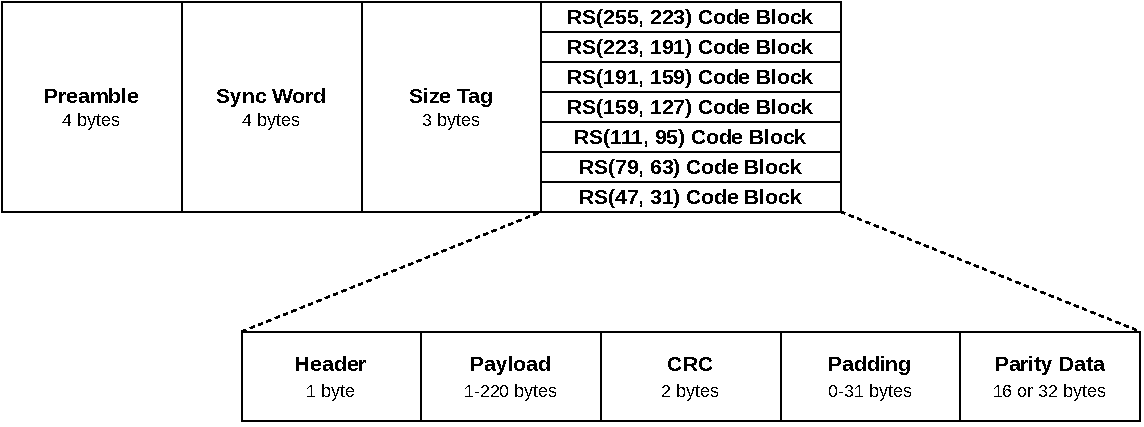
\includegraphics[width=\textwidth]{figures/ngham-pkt.pdf}
        \caption{Format of an NGHam packet.}
        \label{fig:ngham-pkt}
    \end{center}
\end{figure}

Next, there is a brief description of each one of those fields.

\subsubsection{Preamble}

Considering a data rate of 9600 bps, 4 bytes are typically used for the preamble. This sequence is an alternation of ones and zeros: 4$\times$ 0xAA (0b10101010).

\subsubsection{Sync. word}

The sync. word is a sequence of bits used for packet synchronization. With this sequence, the receiver can detect the start of a new packet. In NGHam, the sync. word is composed of 32 bits, following the pattern: 0x5D, 0xE6, 0x2A, 0x7E.

\subsubsection{Size tag}

This field indicates one of the seven possible packet sizes. It is a 24 bits tag and is made very robust by keeping a hamming distance of 13 bits between all vectors. The seven possible tags are listed in \autoref{tab:ngham-sizes}.

\begin{table}[!ht]
    \centering
    \begin{tabular}{llll}
        \toprule[1.5pt]
        \textbf{Size Num.} & \textbf{Tag} & \textbf{Reed-Solomon Config.} & \textbf{Max. Data Size} \\
        \midrule
        1 & 59, 73, 205   & RS(47, 31)   & up to 28 bytes of data \\
        2 & 77, 218, 87   & RS(79, 63)   & up to 60 bytes of data \\
        3 & 118, 147, 154 & RS(111, 95)  & up to 92 bytes of data \\
        4 & 155, 180, 174 & RS(159, 127) & up to 124 bytes of data \\
        5 & 160, 253, 99  & RS(191, 159) & up to 156 bytes of data \\
        6 & 214, 110, 249 & RS(223, 191) & up to 188 bytes of data \\
        7 & 237, 39, 52   & RS(255, 223) & up to 220 bytes of data \\
        \bottomrule[1.5pt]
    \end{tabular}
    \caption{NGHam packets sizes.}
    \label{tab:ngham-sizes}
\end{table}

\subsubsection{Reed-Solomon block}

The Reed-Solomon code block (or just RS block) is the field with packet payload and parity data. It is divided into two parts: data and parity bytes. The data bytes are subdivided into four fields: header, payload, checksum, and padding. Each one of these fields is described below.

\paragraph{Header}

The header byte is the first data byte of the RS block. It is divided as presented in \autoref{tab:ngham-header-flags}.

\begin{table}[!ht]
    \centering
    \begin{tabular}{ll}
        \toprule[1.5pt]
        \textbf{Bits} & \textbf{Purpose} \\
        \midrule
        7 to 6  & Reserved \\
        5       & Extension on \\
        4 to 0  & Padding size (in bytes) \\
        \bottomrule[1.5pt]
    \end{tabular}
    \caption{NGHam header flags.}
    \label{tab:ngham-header-flags}
\end{table}

The extension bit indicates if the extension frame is enabled or not. The padding size bits are the number of padding bytes presented in the respective packet (0 to 31).

\paragraph{Payload}

The payload field is where the “useful” packet data is stored. As presented in the Size Tag field description above, each of the seven size groups allows a maximum number of bytes in the packet payload. The maximum possible length of the payload for an NGHam packet is 220 bytes. If more data need to be transmitted, it should be divided into chunks of 220 bytes and transmitted in separate packets.

\paragraph{Checksum}

There is a checksum field after the payload data to ensure data correctness and a first stage before running the Reed-Solomon correction algorithm. The used checksum algorithm is the CRC16-CCITT 5, with the following configuration:

\begin{itemize}
    \item \textbf{Polynomial}: 0x1021
    \item \textbf{Initial value}: 0xFFFF
    \item \textbf{Final XOR value}: 0xFFFF
\end{itemize}

The CRC16 value is computed from the header and the payload fields.

If the CRC16 value is correct, the Reed-Solomon chain is skipped, and the packet is directly considered valid. This way, the checksum field also allows a performance improvement.

\paragraph{Padding}

To ensure the right packet length for the Reed-Solomon coding in use, if the payload content is less than the maximum allowed, the data field of the RS block is padded with zeros. The number of padding bytes is declared in the header byte (bits 4-0).

\paragraph{Parity data}

This field is reserved for the computed parity bytes of the Reed-Solomon coding algorithm. The used implementation of the RS algorithm is based on the famous FEC library developed by Phil Karn (KA9Q) 6. This field can be 16 or 32 bytes long, depending on the payload length, and consequently, the adopted RS scheme described in \autoref{tab:ngham-parity}.

\begin{table}[!ht]
    \centering
    \begin{tabular}{lll}
        \toprule[1.5pt]
        \textbf{Size Num.} & \textbf{Reed-Solomon Config.} & \textbf{Parity bytes} \\
        \midrule
        1 & RS(47, 31)   & 16 \\
        2 & RS(79, 63)   & 16 \\
        3 & RS(111, 95)  & 16 \\
        4 & RS(159, 127) & 32 \\
        5 & RS(191, 159) & 32 \\
        6 & RS(223, 191) & 32 \\
        7 & RS(255, 233) & 32 \\
        \bottomrule[1.5pt]
    \end{tabular}
    \caption{.}
    \label{tab:ngham-parity}
\end{table}

For the Reed-Solomon framing, the following configuration is used:

\begin{itemize}
    \item \textbf{Symbol size}: 8
    \item \textbf{GF polynomial}: 0x187 (coefficients form)
    \item \textbf{First root of RS code generator polynomial}: 112 (index form)
    \item \textbf{Primitive element}: 11
    \item \textbf{Number of roots}: 16 or 32 (table above)
\end{itemize}

\subsection{Scrambling}

Before transmitting a packet, the RS code block is scrambled by making a byte xor operation with a pre-generated table based on the polynomial $x^{8} + x^{7} + x^{5} + x^{3} + 1$ (defined in the CCSDS 131.0-B-3 standard \cite{ccsds}).

When the receiver receives a packet, it also performs the same operation to de-scramble the RS code block and gets the original content of the RS part of the packet.

By scrambling the packets, long sequences of ones or zeros are avoided by guaranteeing a good bit transition along the whole packet. More information about packet scrambling (or randomization) can be found in \cite{ccsds} (section 8.3).

\section{Flow of execution}
The TTC module operates accordingly to the flowchart from Figure \ref{fig:ttc_flowchart}. Its routine consists of frequent checks for uplink packages or requests from OBDH or EPS to downlink data. Also, by default TTC has protective measures to reset the radio between 600 seconds and the microcontroller after 10 hours.

\begin{figure}[!ht]
    \begin{center}
        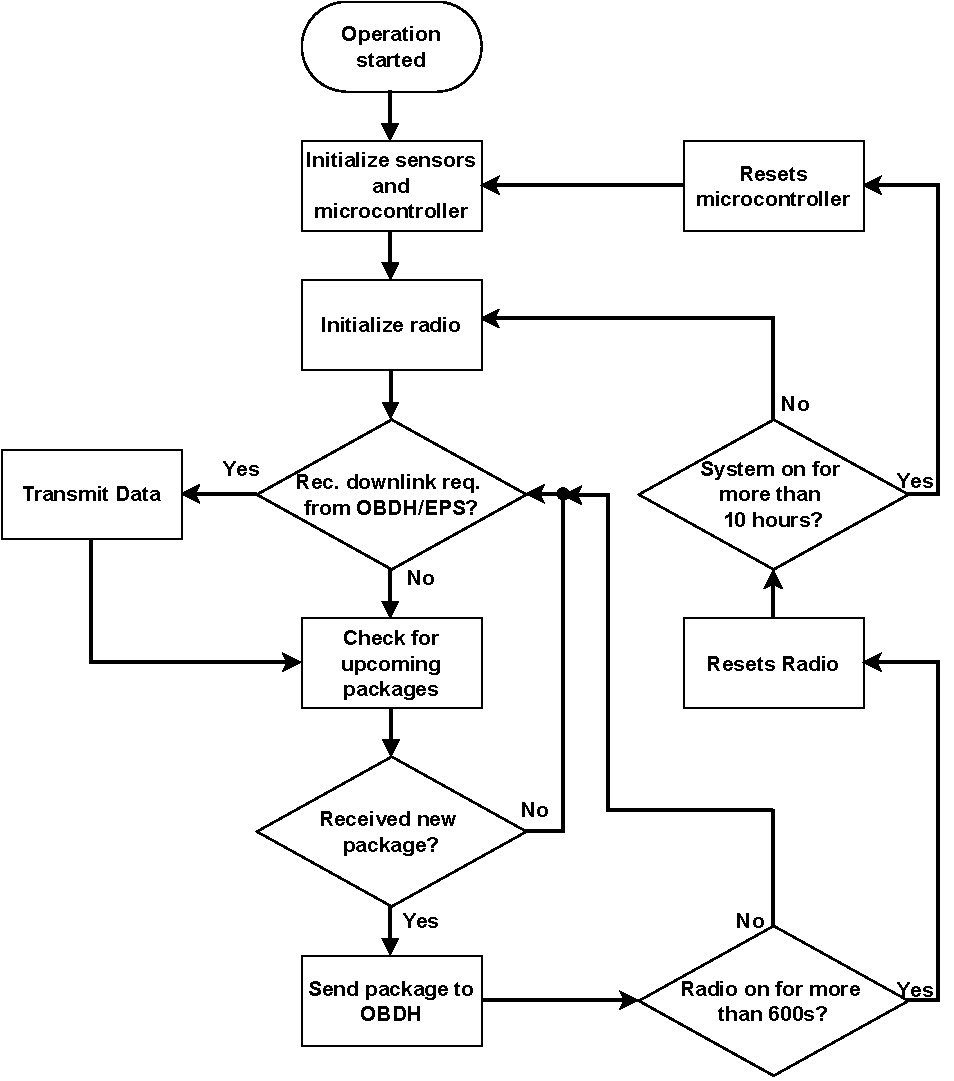
\includegraphics[width=\textwidth]{figures/ttc2-flowchart.pdf}
        \caption{TTC 2.0 flowchart of execution.}
        \label{fig:ttc_flowchart}
    \end{center}
\end{figure}

\section{Server Paramater}

There are two main serial ports accessible to communicate with the TTC module a UART that is accessible only for the radio 1 and can only transmit packages. The other port is an SPI and is possible to communicate individually with each microcontroller and you can requisite all the commands and parameters (see Tables \ref{tab:commands} and \ref{tab:ttc2-variables}). The protocol communication is described below.

\subsection{EPS Server}
The EPS Server is in RX mode and only the Transmit packet command (ID=3) is available. To transmit a package the first byte shall be the command (0x03) followed by the packet. The UART configuration is resumed on Table \ref{tab:eps_config}. This serial port can be accessed via the pin 5 of the PC104-H2 pin 7 is connected to TX but is not utilized, see Table \ref{tab:pc104-pinout}.


\begin{table}[!ht]
    \centering
    \begin{tabular}{clll}
        \toprule[1.5pt]
        \textbf{Configuration Parameter} & \textbf{Value}\\
        \midrule
        Clock               & 1 MHz       \\
        Baud Rate           & 115200 bps  \\
        Data Bits           & 8           \\
        Parity              & No parity   \\
        Stop Bits           & 1           \\
        \bottomrule[1.5pt]
    \end{tabular}
    \caption{EPS Server configuration parameter.}
    \label{tab:eps_config}
\end{table}

\begin{figure}[!ht]
    \begin{center}
        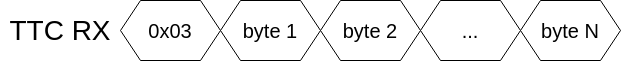
\includegraphics[width=0.5\textwidth]{figures/eps_communication.drawio.png}
        \caption{EPS Server communication diagram description.}
        \label{fig:eps-server-communication}
    \end{center}
\end{figure}

\subsection{OBDH Server}
The OBDH Server can be used for full communication and all the commands are implemented for this port. The TTC operates as half-duplex with the commands having a request and a followed by response (except for command Write parameter ID=2 that only uses a request). For commands that need a response it is required to leave a interval of at least 100ms from the request to the response. Each communication part, for both sides, in all commands starts with the preamble byte (0x7E) that can be used to detect and sincronize wrong transactions. When each side is communicating the listening side needs to send 0x00 while the other side transmits.
All the request have seven bytes length including the preamble, the response for command ID=1 also has 7 bytes as fixed size, the response from commands ID=3 and ID=4 have a variable size accordingly to the request. The communication for each case is described in Figure \ref{fig:obdh-server-communication}. The TTC operates in spi mode 0 and was tested with 1 MHz clock.

\begin{figure}[!ht]
    \begin{center}
        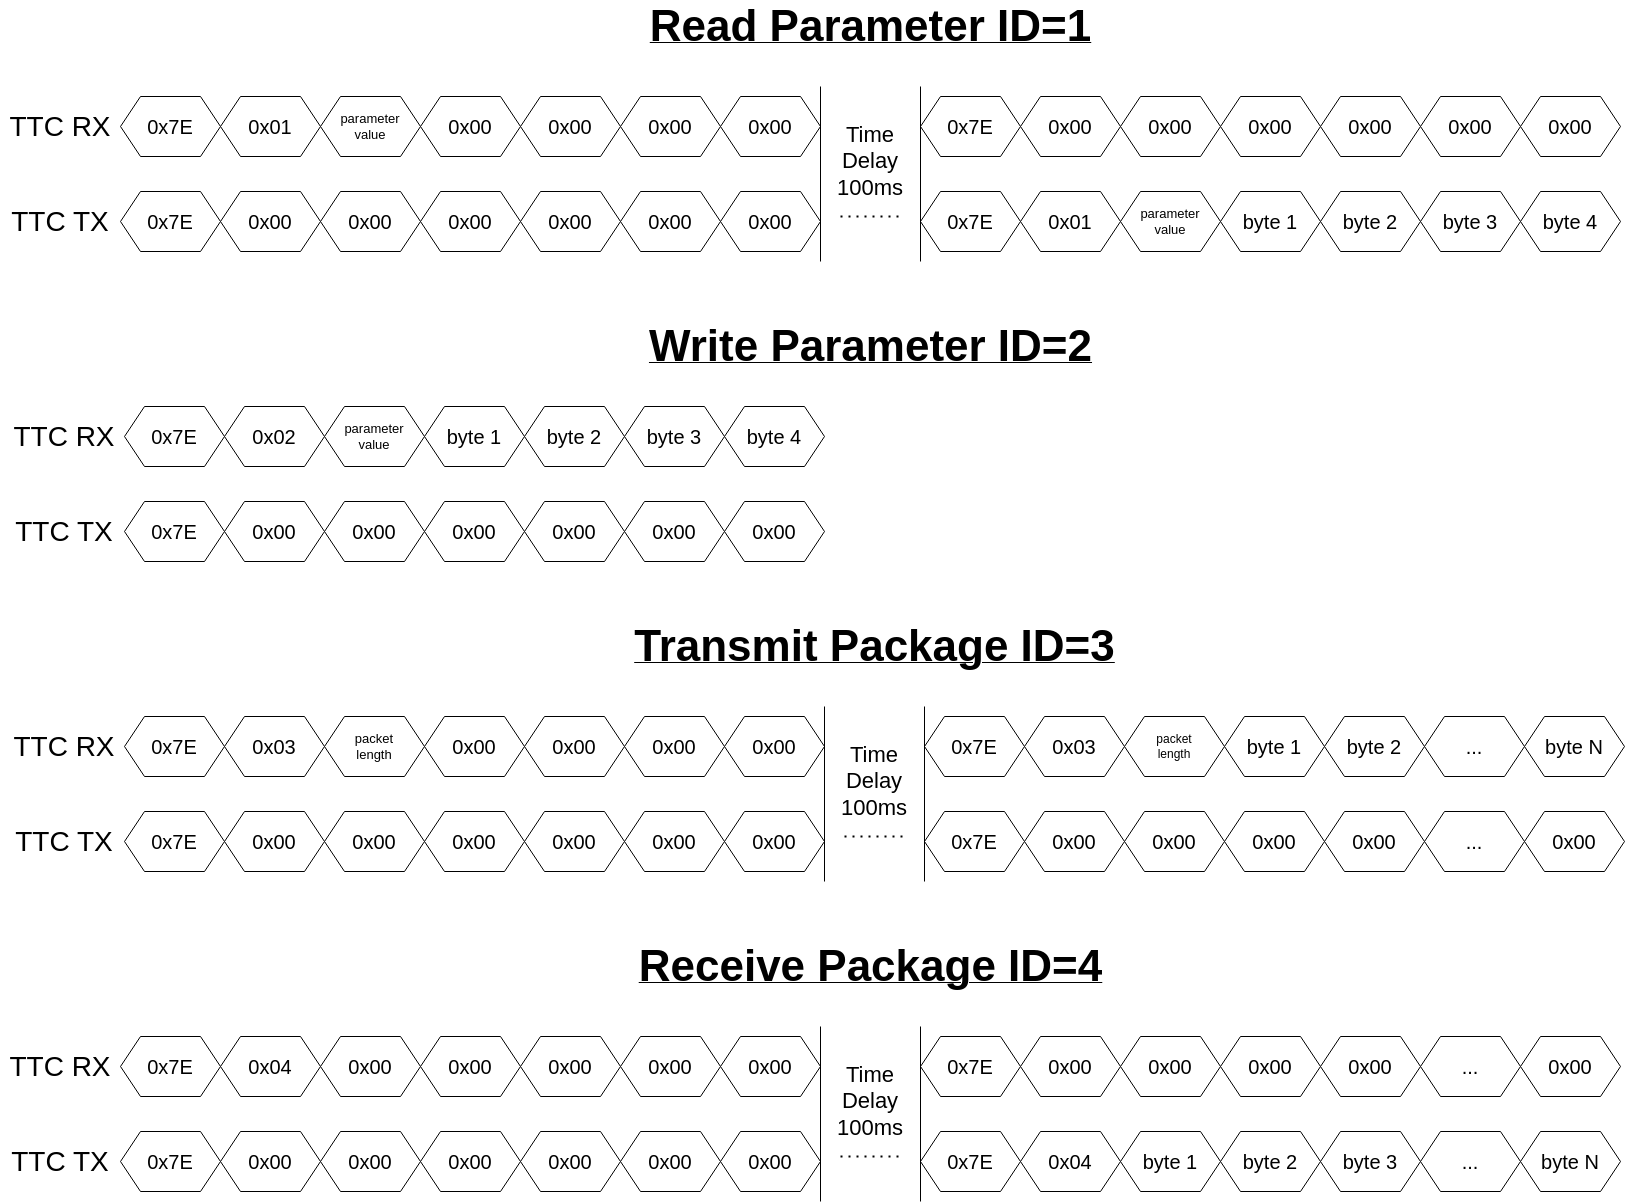
\includegraphics[width=1\textwidth]{figures/obdh_communication.drawio.png}
        \caption{OBDH Server communication diagram description.}
        \label{fig:obdh-server-communication}
    \end{center}
\end{figure}

\begin{table}[!ht]
    \centering
    \begin{tabular}{clll}
        \toprule[1.5pt]
        \textbf{Configuration Parameter} & \textbf{Value}\\
        \midrule
        Mode                & 0                 \\
        Clock               & 200 kHz to 1 MHz  \\
        \bottomrule[1.5pt]
    \end{tabular}
    \caption{OBDH Server configuration parameter.}
    \label{tab:eps_config}
\end{table}

    \section{Documentation}

        %
% documentation.tex
%
% Copyright (C) 2022 by SpaceLab.
%
% TTC 2.0 Module
%
% This work is licensed under the Creative Commons Attribution-ShareAlike 4.0
% International License. To view a copy of this license,
% visit http://creativecommons.org/licenses/by-sa/4.0/.
%

%
% \brief Documentation slides.
%
% \author Gabriel Mariano Marcelino <gabriel.mm8@gmail.com>
% \author Miguel Boing <miguelboing13@gmail.com>
%
% \version 0.1.0
%
% \date 2022/08/07
%


\begin{frame}{Documentation}

    \begin{itemize}
        \item User manual (PDF)
        \vspace{0.4cm}
        \item This presentation
        \vspace{0.4cm}
        \item Schematics
        \vspace{0.4cm}
        \item Firmware: Doxygen
    \end{itemize}

\end{frame}

    \section{Management}

        %
% management.tex
%
% Copyright (C) 2022 by SpaceLab.
%
% TTC 2.0 Critical Design Review
%
% This work is licensed under the Creative Commons Attribution-ShareAlike 4.0
% International License. To view a copy of this license,
% visit http://creativecommons.org/licenses/by-sa/4.0/.
%

%
% \brief Project management slides.
%
% \author Gabriel Mariano Marcelino <gabriel.mm8@gmail.com>
% \author Miguel Boing <miguelboing13@gmail.com>
%
% \version 0.1.0
%
% \date 2022/07/28
%


\begin{frame}{Project Management}

    \begin{itemize}
        \item Activities and tasks: Public GitHub issues/project
        \vspace{0.25cm}
        \item Source files and versioning control: \href{https://github.com/spacelab-ufsc/obdh2}{\textcolor{blue}{Git repository}} with three development branches:
            \begin{itemize}
                \item \textit{dev\_doc}: Documentation
                \item \textit{dev\_hardware}: Hardware project
                \item \textit{dev\_firmware}: Firmware project
            \end{itemize}
    \end{itemize}

    \begin{figure}[!ht]
        \begin{center}
            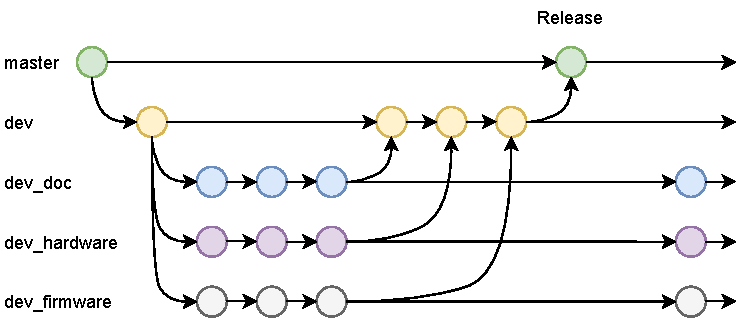
\includegraphics[width=7cm]{figures/git-flow.pdf}
        \end{center}
    \end{figure}

\end{frame}

    \sectionpic{Thanks!}{figures/brazil-south.jpeg}

\end{document}
